\documentclass[11pt, letterpaper]{article}
\input{/home/hyperion/.config/LatexHub/preambles/base.tex}
\input{/home/hyperion/.config/LatexHub/preambles/diagrams.tex}
\input{/home/hyperion/.config/LatexHub/preambles/tikz.tex}
\input{/home/hyperion/.config/LatexHub/preambles/macros-cat-theory.tex}
\input{/home/hyperion/.config/LatexHub/preambles/macros-algebra.tex}
\input{/home/hyperion/.config/LatexHub/preambles/basic-theorems-section.tex}
\input{/home/hyperion/.config/LatexHub/preambles/refs-basic.tex}
\theoremstyle{plain}
\newtheorem{problem}{Problem}
\usepackage{titlepageBU}
\title{Weight decomposition for semi-simple Lie algebra}
\begin{document}
\makeproblem

\begin{problem}
	Let $V$ be the vector space of homogeneous polynomials of degree 3 in variables $x,y,z$, equipped with the natural action of $\mathfrak{sl} _3(\mathbb{C} )$. 
	\begin{enumerate}
		\item Let
			\[
				\mathfrak{h} =\left\{ \operatorname{diag} (h_1,h_2,h_3)\mid h+1h_2+h_3=0 \right\} \subseteq \mathfrak{sl} _3(\mathbb{C} )
			.\]
			Write down the root space decomposition of $\mathfrak{sl} _3(\mathbb{C} )$ with respect to $\mathfrak{h} $.
		\item For each simple root, write down the corresponding $\mathfrak{sl} _2$-triples explicitly as $3\times 3$ matrices.
		\item Write down explicitly the action of $\mathfrak{sl} _3(\mathbb{C} )\subseteq \mathfrak{gl} _3(\mathbb{C} )$ on $V$.
		\item Compute the weight decomposition of $V$ with respect to $\mathfrak{h} $. List all weights and their multiplicities.
		\item Draw the weight lattice for this representation, indicating all weights and their multiplicities.
		\item Choose one of the $\mathfrak{sl} _2$-triples and compute explicitly how it acts on the monomial basis $x^ay^bz^c$. Describe the resulting $\mathfrak{sl} _2$-strings in $V$.
		\item Describe the Weyl group of $\mathfrak{sl} _3(\mathbb{C} )$ and compute its action on the weight lattice. Verify that the set of weights is invariant under this action and determine the Weyl group orbits.
	\end{enumerate}
\end{problem}
\begin{proof}
	(1) Let $h=\operatorname{diag} (h_1,h_2,h_3)\in \mathfrak{h} $. The linear functionals $\mathfrak{h} ^*$ are generated by $L_ih=h_i$, $1\leq i\leq 3$. Let $E_{ij} =\delta _i^j $ denote the standard basis matrices of $\mathfrak{gl} _3(\mathbb{C} )$. Then note that $[h,E_{ij} ]=(h_i-h_j)E_{ij} $. Rewite this as
	\[
		[h,E_{ij} ]=(L_ih - L_jh)E_{ij} = (L_i-L_j)(h)E_{ij} 
	.\]
	Thus we find that the roots are generated by $L_i-L_j$, and that the root space $\mathfrak{g} _{L_i-L_j} $ is $\operatorname{span} (E_{ij})$ as a $\mathbb{C} $-vector space. The root space decomposition is
	\[
		\mathfrak{sl} _3(\mathbb{C} )=\mathfrak{h} \oplus \bigoplus_{1\leq i\neq j \leq 3} \mathfrak{g} _{L_i-L_j} .
	\]
	
	(2) Write $\alpha _1 = L_1-L_2$, $\alpha _2=L_2-L_3$, and $\alpha _3=L_1-L_3$. We claim the simple roots are $L_1 - L_2$ and $L_2-L_3$. This is immediately shown: $\left\{ \alpha _1,\alpha _2 \right\} $ clearly forms a basis for $\mathfrak{h} ^*$, and additionally, $\alpha_3 = \alpha _1 + \alpha _2$.

	We now find the $\mathfrak{sl} _2$-triples for the simple roots. Since $\mathfrak{g} _{\alpha _1} =\operatorname{span} (E_{12} )$, we set $e_1=cE_{12} $ for some $c\in\mathbb{C}^\times $. Similarly, $\mathfrak{g} _{-\alpha _1} =\operatorname{span} (E_{21} )$ implies $f_1 = dE_{21} $ for some $d\in\mathbb{C} ^{\times } $. We use the $\mathfrak{sl} _2$ commutator relations to compute
	\[
		h_1 = [e_1,f_1]=cd\left( E_{12} E_{21} -E_{21} E_{12}  \right) =cd\left( E_{11} -E_{22}  \right) 
	.\]
	Note that $h_1\in \mathfrak{h} $ implies $\alpha _1(h_1)e_1 = [h_1,cE_{12} ]=2e_1$, and thus $\alpha_1(h_1)=2$. It follows that
	\[
		2=\alpha _1(h_1) = cd\left(L_1(E_{11} ) - L_2(E_{22} )\right) = 2cd
	.\]
	We set $c=d=1$. This yields
	\[
		e_1 = E_{12} =\begin{pmatrix}
		0 & 1 & 0 \\
		0 & 0 & 0 \\
		0 & 0 & 0
		\end{pmatrix},\qquad f_1=E_{21} =\begin{pmatrix}
		0 & 0 & 0 \\
		1 & 0 & 0 \\
		0 & 0 & 0
		\end{pmatrix},\qquad h_1 = \begin{pmatrix}
		1 & 0 & 0 \\
		0 & -1 & 0 \\
		0 & 0 & 0
		\end{pmatrix}
	.\]
	The same logic shows that $e_2 = E_{23} $, $f_{2} =E_{32} $, and $h_2 = E_{22} -E_{33} $. Thus
	\[
		e_2 = \begin{pmatrix}
		0 & 0 & 0 \\
		0 & 0 & 1 \\
		0 & 0 & 0
		\end{pmatrix},\qquad f_2 = \begin{pmatrix}
		0 & 0 & 0 \\
		0 & 0 & 0 \\
		0 & 1 & 0
		\end{pmatrix},\qquad h_2 = \begin{pmatrix}
		0 & 0 & 0 \\
		0 & 1 & 0 \\
		0 & 0 & -1
		\end{pmatrix}
	.\]
	
	(3) We start with the obvious representation on $\mathbb{C} ^3 = \operatorname{span} \left\{ x_1,x_2,x_3 \right\} $ given by matrix multiplication $E_{ij} x_k=\delta _{jk} x_i$. Then we note that $V$ is the third symmetric power $V \cong \Sym^3\left( \mathbb{C} ^3\right)$, and we can extend Lie algebra actions to symmetric powers by acting as derivations:
	\[
		X(pq) = X(p)q + pX(q),\qquad X\in \mathfrak{sl} _3(\mathbb{C} ),\,\, p,q\in\mathbb{C} ^3
	.\]
	The Leibniz rule implies that $\mathfrak{sl} _3(\mathbb{C} )$ should act via differential operators. We start by noting that $E_{ij}\cdot x_k = \delta _{jk} x_i = x_i \partial _jx_k$. Since derivatives satisfy the Leibniz rule, this extends naturally to the symmetric power $V$. Thus we can define the action of $E_{ij} $ on $V$ by
	\[
		E_{ij} p = x_i \frac{\partial p}{\partial x_j} ,\qquad p\in V
	.\]
	We then of an arbitrary $X\in \mathfrak{sl} _3(\mathbb{C} )$ on $p\in V$ by noting that $\left\{ E_{ij}  \right\} _{1\leq i,j\leq 3} $ is a basis for $\mathfrak{sl} _3(\mathbb{C} )$.

	(4) The space $V$ has a basis $B=\left\{ x^ay^bz^c \mid a+b+c=3,\;\; a,b,c\geq 0 \right\} $ of degree 3 monomials. Let $h=\operatorname{diag} (h_1,h_2,h_3)\in \mathfrak{h} $. Then by (3),
	\[
		h\cdot x^ay^bz^c = \left( h_1 x\frac{\partial }{\partial x} + h_2 y\frac{\partial }{\partial y} + h_3 z\frac{\partial }{\partial z}  \right) \left( x^ay^bz^c \right) =\left( ah_1+bh_2+ch_3 \right) x^ay^bz^ch
	.\]
	This corresponds to a weight $\lambda_{a,b,c}  =aL_1 + bL_2 + cL_3$, since $\lambda _{a,b,c} (h) x^ay^bz^c= h\cdot x^ay^bz^c$. Each tuple $(a,b,c)$ of nonnegative integers thus determines a unique weight, meaning all weights have a multiplicity of 1.

	(5) See \cite{fig:1}, which is on the next page due to LaTeX figure placement being trash. Warning: I cannot draw well.
	\begin{figure}[ht]
		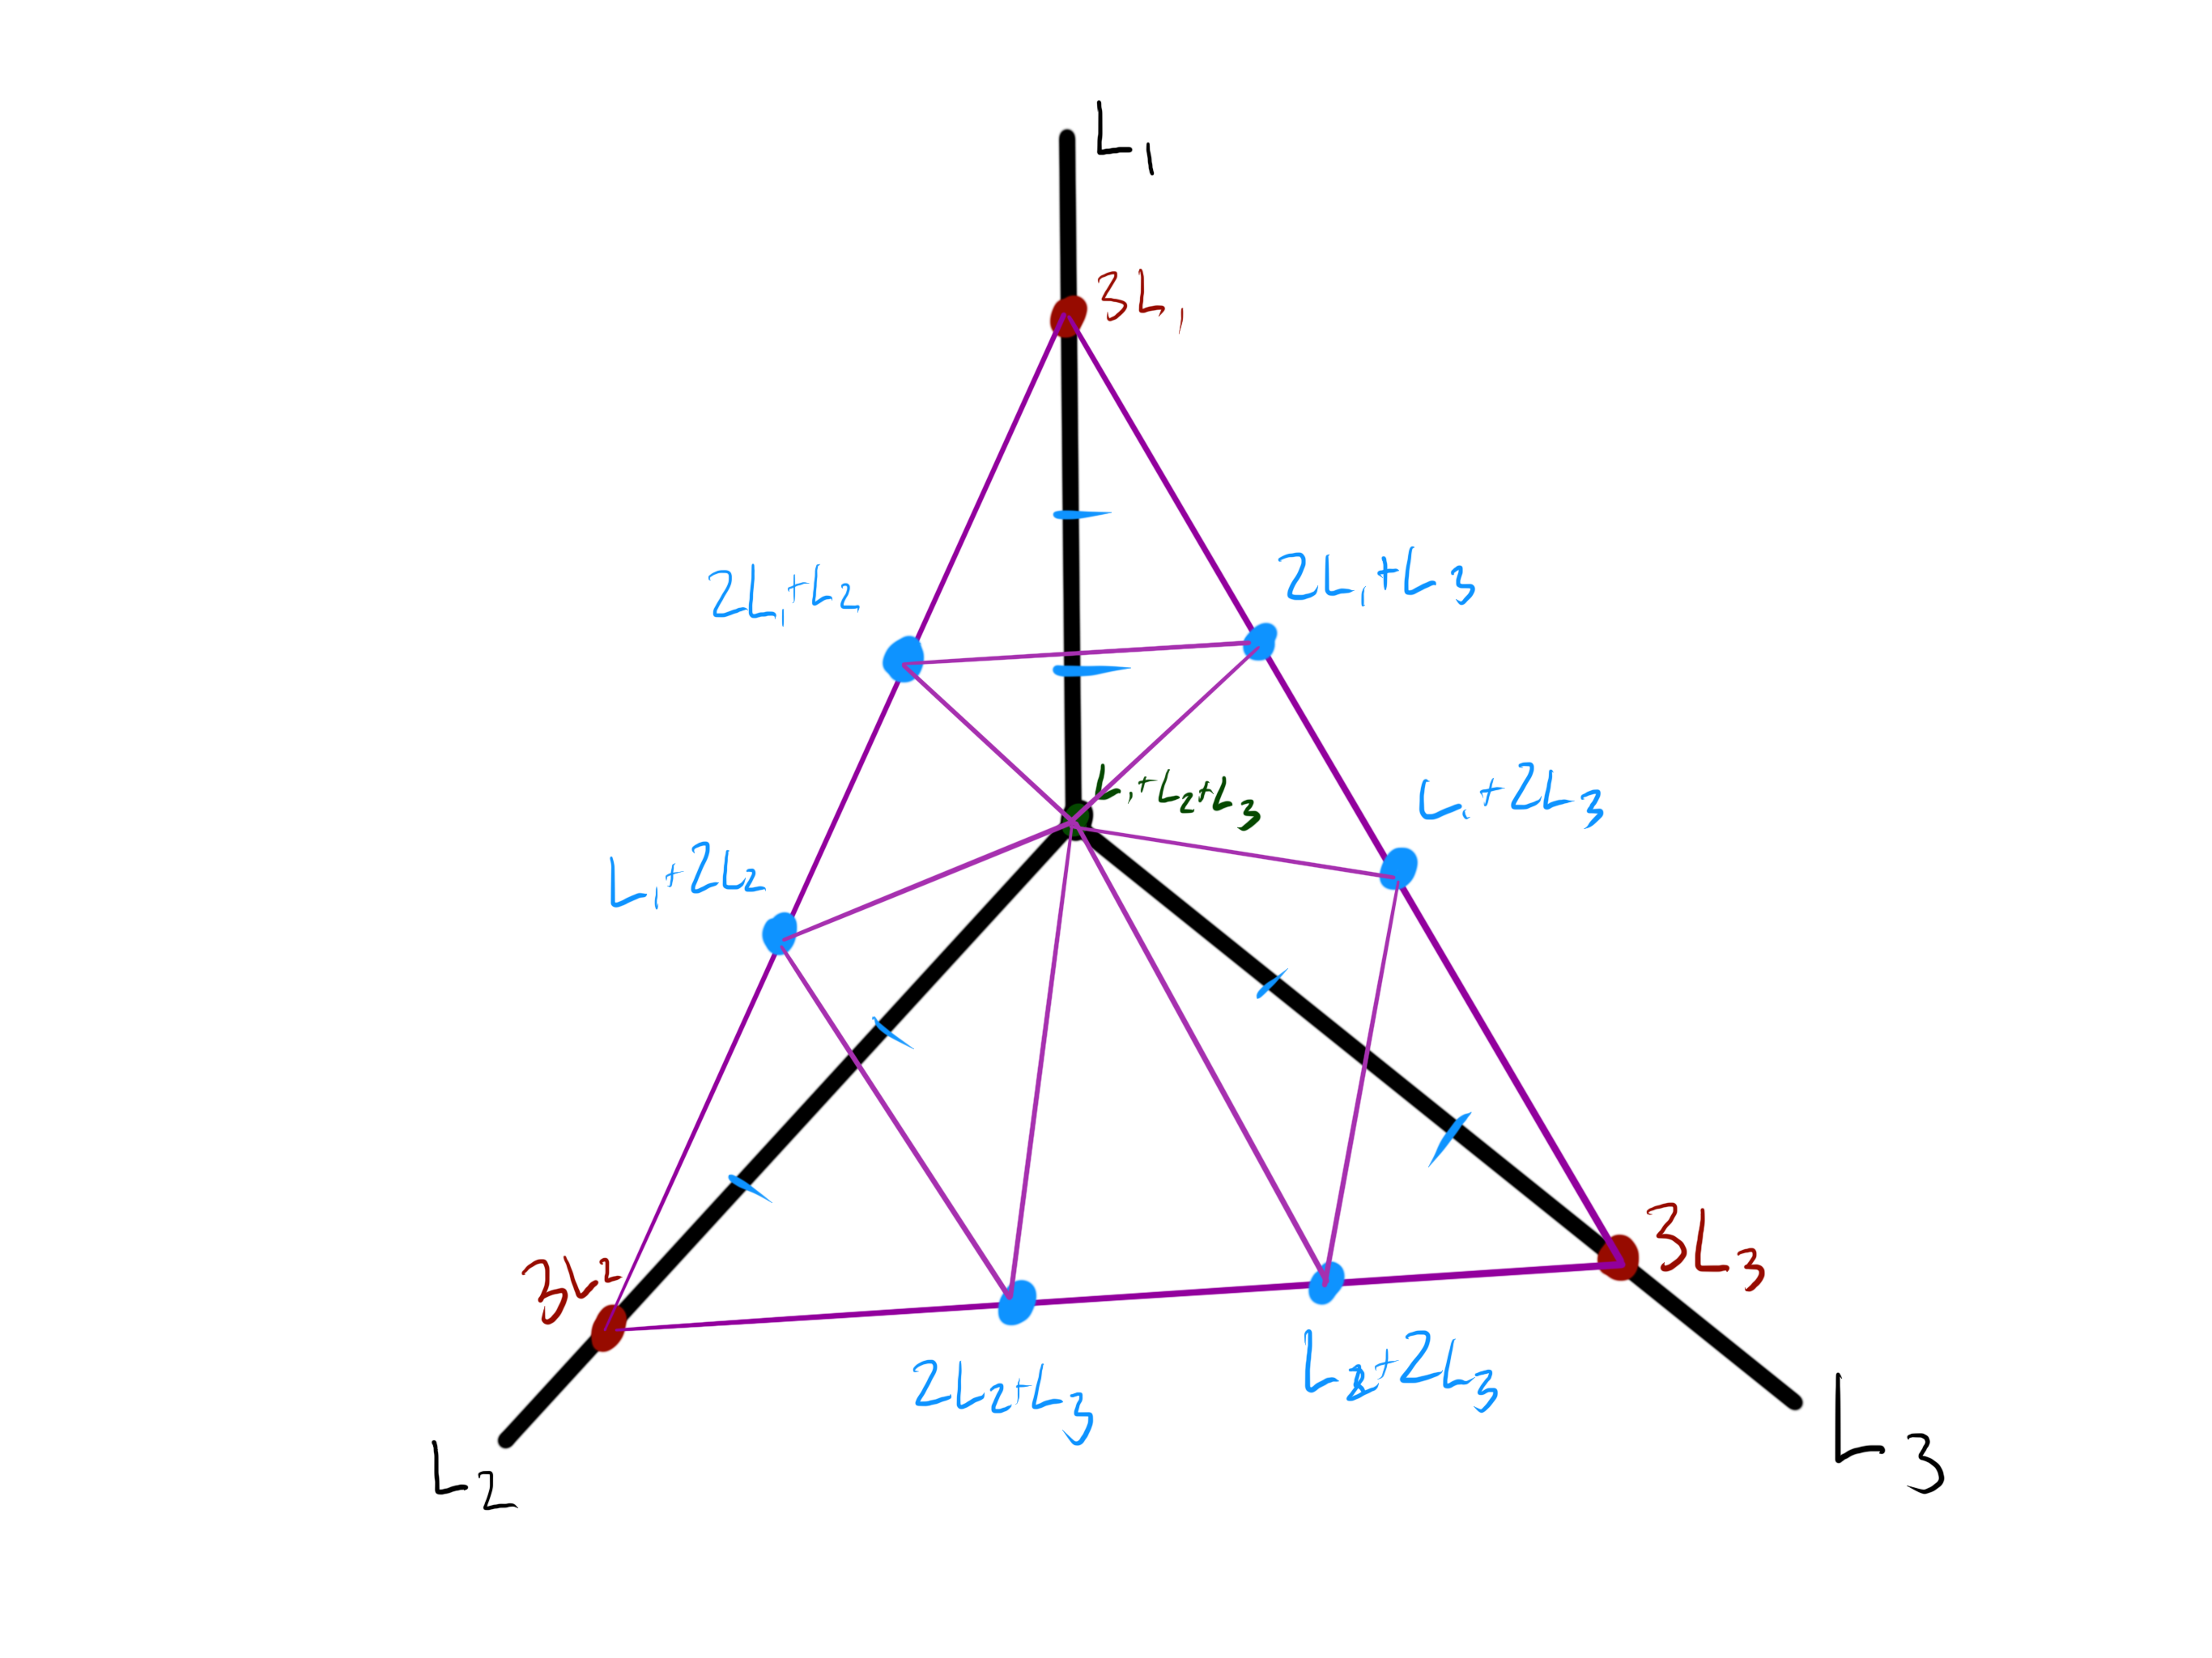
\includegraphics[scale=0.25]{../figures/weight.jpg}
		\centering
		\caption{Weight lattice for $\mathfrak{sl} _3(\mathbb{C} )$}\label{fig:1}
		\centering
	\end{figure}
	

	(6) Consider the $\alpha _1$ $\mathfrak{sl} _2$-triple $(e_1,f_1,h_1)$. As polynomial differential operators these are
	\[
		e_1 = x \frac{\partial }{\partial y} ,\qquad f_1 = y \frac{\partial }{\partial x} ,\qquad h_1 = x \frac{\partial }{\partial x} - y \frac{\partial }{\partial y} 
	.\]
	This yields
	\[
		e_1\cdot x^ay^bz^c = bx^{a+1} y^{b-1} z^c,\qquad f_1\cdot x^ay^bz^c = a x^{a-1} y^{b+1} z^c,
	\]
	\[
		h_1\cdot x^ay^bz^c = (a-b)x^ay^bz^c
	.\]
	I assume $\mathfrak{sl} _2$-strings are given by applying the raising and lowering operators, so we compute those for $\alpha _1$. Since this $\mathfrak{sl} _2$-action leaves the $z^c$ component invariant, there are four strings as follows.
	\begin{itemize}
		\item $(c=0)$ There is a 4-dimensional string
			\[\begin{tikzcd}[row sep = 2.5em, column sep = 2.5em]
			\left\langle y^3 \right\rangle \ar[" e_1 ", shift left, r]  & \left\langle xy^2 \right\rangle \ar[" e_1 ", shift left, r] \ar[" f_1 ", shift left, l]  & \left\langle x^2y \right\rangle \ar[" e_1 ", shift left, r] \ar[" f_1 ", shift left, l]  & \left\langle x^3 \right\rangle \ar[" f_1 ", shift left, l] .
			\end{tikzcd}\]
			This string has highest weight 3.
		\item $(c=1)$ There is a 3-dimensional string
			\[\begin{tikzcd}[row sep = 2.5em, column sep = 2.5em]
			\left\langle x^2z \right\rangle \ar[" e_1 ", shift left, r]  & \left\langle xyz \right\rangle \ar[" e_1 ", shift left, r] \ar[" f_1 ", shift left, l]  & \left\langle y^2z \right\rangle \ar[" f_1 ", shift left, l] .
			\end{tikzcd}\]
			This string has highest weight 2.
		\item $(c=2)$ There is a 2-dimensional string
			\[\begin{tikzcd}[row sep = 2.5em, column sep = 2.5em]
			\left\langle xz^2 \right\rangle \ar[" e_1 ", shift left, r]  & \left\langle yz^2 \right\rangle \ar[" f_1 ", shift left, l] .
			\end{tikzcd}\]
			This string has highest weight 1.
		\item $(c=3)$ Since $z^3$ is annihilated by $e_1$ and $f_1$, we have that $\left\langle z^3 \right\rangle $ is a trivial 1-dimensional $\mathfrak{sl} _2$-string of highest weight 0.
	\end{itemize}
	
	(7) We use the inner product $\left\langle L_i,L_j \right\rangle =\delta _{ij} $ to prove that the Weyl group of $\mathfrak{sl} _3(\mathbb{C} )$ is isomorphic to $S_3$. The Weyl group is generated by relections
	\[
		s_\alpha (\lambda )=\lambda -\frac{2\left\langle \lambda ,\alpha  \right\rangle }{\left\langle \alpha ,\alpha  \right\rangle } \alpha ,
	\]
	where $\alpha $ is a simple root and $\lambda \in \mathfrak{h} ^*$. First, note that
	\[
		\left\langle \alpha_1,\alpha _1 \right\rangle =\left\langle L_1-L_2,L_1-L_2 \right\rangle =2,
	\]
	\[
		\left\langle \alpha _2,\alpha _2 \right\rangle =\left\langle L_2-L_3,L_2-L_3 \right\rangle =2
	.\]
	Thus $s_\alpha (\lambda )=\lambda -\left\langle \lambda ,\alpha  \right\rangle \alpha $. Let $\lambda =aL_1+bL_2+cL_3\in \mathfrak{h} ^*$. Then we compute
	\[
		\left\langle \lambda ,\alpha _1 \right\rangle =a-b,\qquad \left\langle \lambda ,\alpha _2 \right\rangle =b-c
	.\]
	Thus
	\[
		s_{\alpha _1} (\lambda )=aL_1 + bL_2 + cL_3 - (a-b)(L_1 - L_2) = aL_1 + bL_2 + cL_3 - aL_1 + bL_1 + aL_2 - bL_2
	\]
	\[
		=bL_1 + aL_2 + cL_3
	;\]
	\[
		s_{\alpha _2} (\lambda ) = aL_1 + bL_2 + cL_3 - bL_2 + cL_2 + bL_3 - cL_3 = aL_1 + cL_2 + bL_3
	.\]
	We thus find that if we write $\lambda (a,b,c)$ as a vector in the $\left\{ L_i \right\} $-basis, then the Weyl group $W$ is isomorphic to the symmetric group $S_3$: $s_{\alpha _1} $ acts as the transposition $(12)$, $s_{\alpha _2} $ acts as the transposition $(23)$, and these two elements generate $S_3$ (note that $(12)(23)=(123)$ so you get 3-cycles).

	With this in mind, we consider the action of $W\cong S^3$ on the weight lattice $\Pi $. Recall that weights are $\Pi \ni\lambda =aL_1 + bL_2 + cL_3 = (a,b,c)$ with $a+b+c=3$ nonnegative integers. If we permute the indicies, then they are still all nonnegative and still sum to 3, so $S_3\Pi  \subseteq \Pi $. There are three distinct orbits.

	\begin{itemize}
		\item If $(a,b,c) = (3,0,0)$, then the orbit of $\lambda $ is $\left\{ (3,0,0),(0,3,0),(0,0,3) \right\} $. Explicitly, this is $\left\{ 3L_1,3L_2,3L_3 \right\} $.
		\item If $(a,b,c) = (2,1,0)$, then the orbit of $\lambda $ is all permutations of $(2,1,0)$:
			\[
				\left\{ 2L_1 + L_2, 2L_1 + L_3, L_1 + 2L_2, 2L_2 + L_3, L_1 + 2L_3, L_2 + 2L_3 \right\} 
			.\]
		\item If $(a,b,c) = (1,1,1)$,  then the orbit of $\lambda $ is the only permutation of $(1,1,1)$: $\left\{ L_1 + L_2 + L_3 \right\} $.
	\end{itemize}
\end{proof}


\end{document}
